	\chapter{Introdução}

Desde a década de 60, robôs tem sido utilizados em ambientes industriais. Manipuladores robóticos foram capazes de aumentar a produtividade, a eficiência e garantir um maior controle de qualidade dos processos. Além de serem capazes de realizar tarefas repetitivas em uma linha de montagem, muitos manipuladores o fazem com maior precisão e rapidez que um ser humano. 

Recentemente além de linhas de produção da industria, a robótica tem encontrado aplicação em instalações \textit{offshore} de óleo e gás. É de grande interesse utilizá-los para realizar tarefas onde a presença humana torna-se difícil, arriscada ou até mesmo impossível. Muitas empresas já tem utilizado soluções automatizadas tanto em ambientes submersos quanto acima do nível do mar. Braços robóticos tem sido de grande importância para executar tarefas que exigem interação mais complexa com o ambiente. Com isso em mente, foi desenvolvido um manipulador leve para o DORIS, robô guiado por trilhos para monitoração, inspeção e supervisão de ambientes não submersos de plataformas de petróleo \citep{xaud2016doris}.

\section{Motivação}
\subsection{Robótica em instalações \textit{offshore}}
O setor de óleo e gás tem crescido constantemente, com a produção sendo gradualmente expandida até locais não explorados e inacessíveis. As condições de trabalho encontradas em geral nesses locais incluem chuvas pesadas, vento, temperaturas extremas, ambiente explosivo, corrosivo e produtos químicos tóxicos. Nesse cenário, empresas de óleo e gás tem investido no desenvolvimento de tecnologias que permitam a produção nesses ambientes. Com isso, a aplicação de automação de processos e robótica tem crescido rapidamente. Robôs tem sido utilizados para tarefas de inspeção, manutenção, reparo e supervisão de instalações \textit{offshore}, aumentando a eficiência dos processos, a segurança e saúde dos funcionários, além de diminuir os custos de operação e logística.  

O uso de robôs instalações de óleo e gás tem diversas vantagens \citep{skourup2009robotized}. Pode reduzir o custo com manutenção de múltiplos sensores ao longo instalação e substituir humanos na realização de tarefas repetitivas, especialmente aquelas realizadas em ambientes perigosos, confinados ou prejudiciais a saúde. 

Hoje a maioria dos robôs utilizados no setor de óleo e gás é composta de Veículos Operados Remotamente (ROVs\footnotemark[1]) e Veículos Submarinos Autônomos (AUVs \footnotemark[2]), utilizados para operações submarinas como mapeamento do solo oceânico, perfuração, inspeção e reparo de equipamento submarino, tubulações, âncoras, entre outros. No entanto, pesquisas atuais tem focado também em aplicações de robótica na área \textit{topside} das plataformas, buscando realizar tarefas como:
\begin{itemize}
\item Monitorar indicadores de processos.
\item Supervisionar o bom funcionamento máquinas e equipamentos.
\item Detectar o vazamento de gás ou fluido, anomalias, fogo e fumaça.
\item Manipular válvulas, botões e alavancas.
\item Supervisão de pessoal não autorizado e objetos.
\end{itemize} 


\footnotetext{ROV do inglês Remotely Operated underwater Vehicle}
\footnotetext{AUV, do inglês Autonomous Underwater Vehicle}

\newlength{\tsub}
\newsavebox{\tsubbox}

\begin{figure}[htp]
% preliminary
\sbox\tsubbox{%
  \resizebox{\dimexpr.9\textwidth-1em}{!}{%
    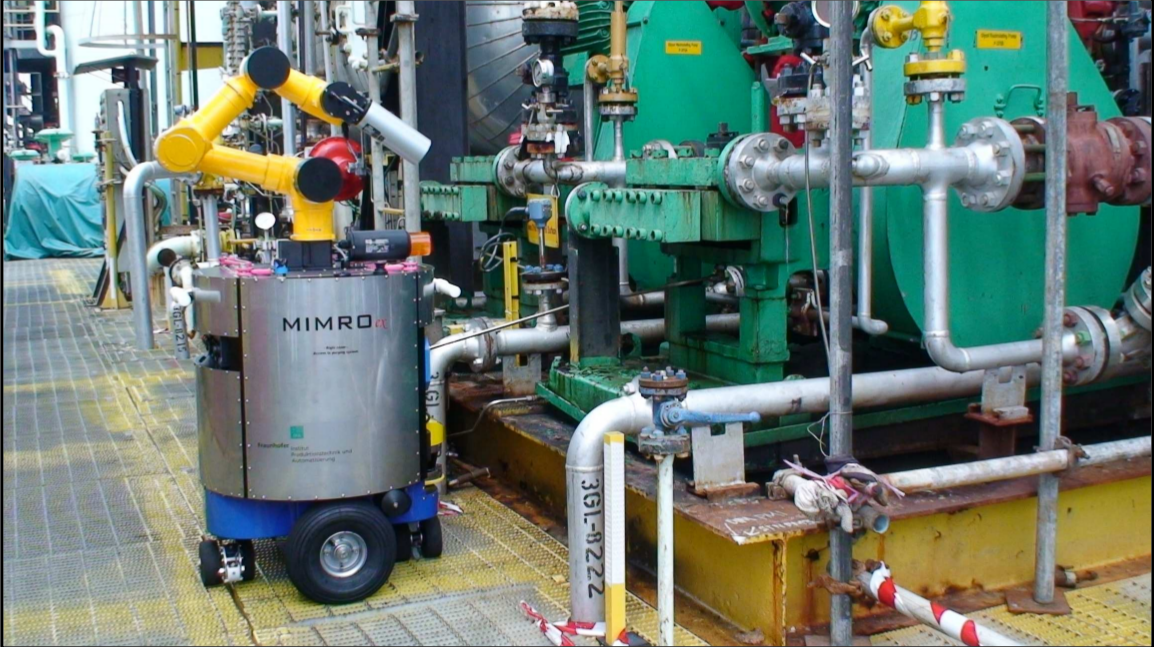
\includegraphics[height=3cm]{./img/mimro.png}%
    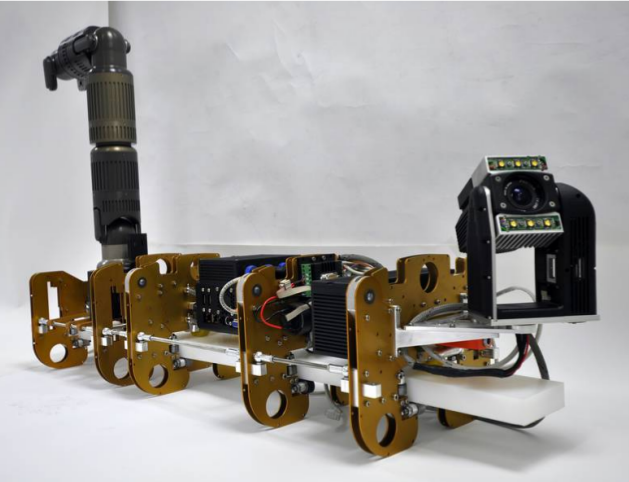
\includegraphics[height=3cm]{./img/artis.png}%
  }%
}
\setlength{\tsub}{\ht\tsubbox}
% typeset
\centering
\subcaptionbox{MIMROex\label{fig:mimro}}{%
  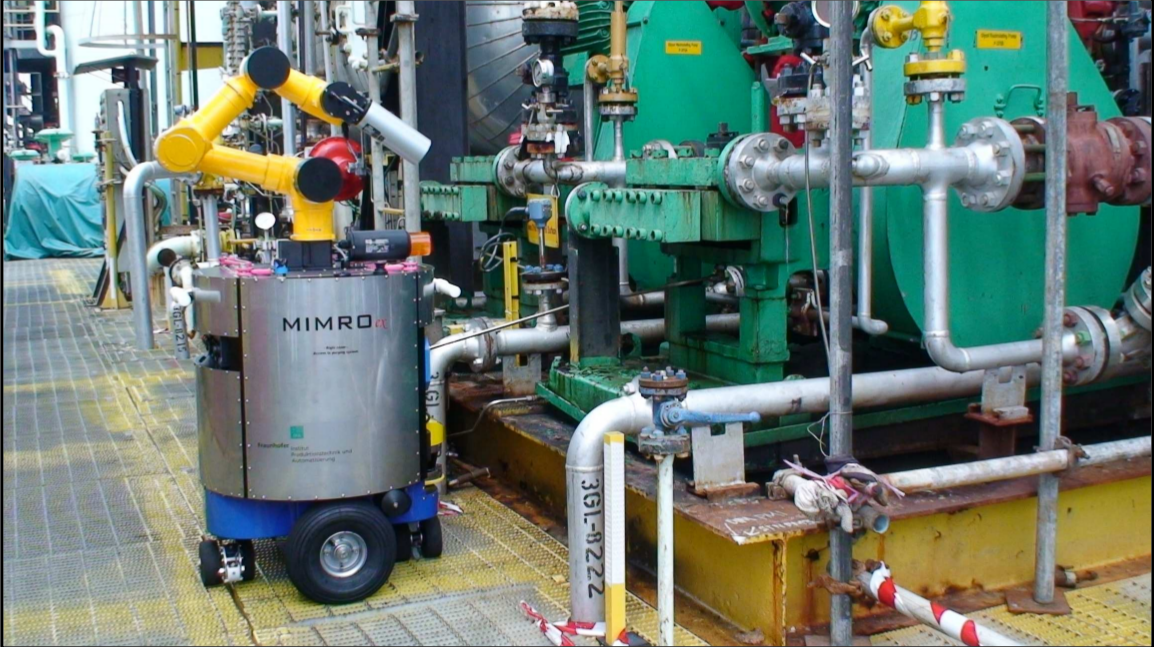
\includegraphics[height=\tsub]{./img/mimro.png}%
}\quad
\subcaptionbox{ARTIS\label{fig:artis}}{%
  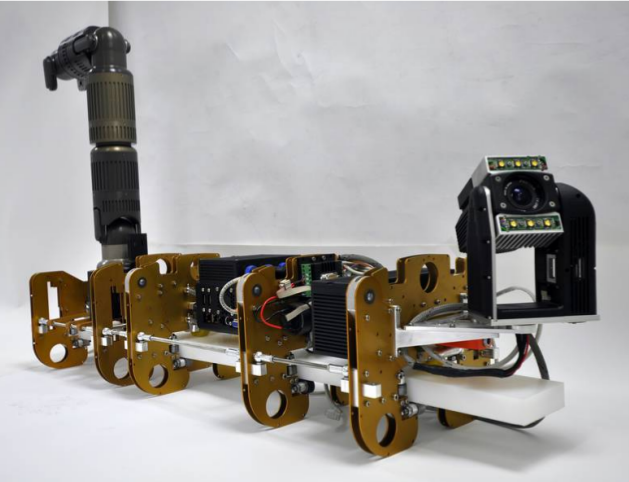
\includegraphics[height=\tsub]{./img/artis.png}%
}
\caption{MIMROex e ARTIS}
\end{figure}

Dentre os robôs para áreas \textit{topside} de plataformas, podemos mencionar o MIMROex, desenvolvido pela Fraunhoffer IPA para tarefas de inspeção e monitoração \citep{bengel2007mimroex}, mostrado na Figura \ref{fig:mimro}.

Robôs como esse movem-se ao longo da plataforma e possuem muitos graus de liberdade, tornando seu projeto de controle bastante complexo. Portanto, foram propostas soluções como o ARTIS, \textit{Autonomous Railguided Tank Inspection System} \citep{artis} da DFKI (\textit{German Research Center for Artificial Intelligence}). Esse robô se move de forma restrita a um trilho que é projetado de forma a levá-lo até todos os pontos de interesse, isso diminui a complexidade do projeto. 


O robô Sawyer\texttrademark, mostrado na Figura \ref{fig:sawyer}, é a segunda geração de robôs de alto desempenho desenvolvidos pela Rethink Robotics$^\circledR$, é projetado par trabalhar lado a lado com humanos \citep{ieee2015sawyer}. Algumas de suas especificações são mostradas na tabela 


\begin{table}[h!]
\centering
\caption{Especificações do Rethink Robotics$^\circledR$ Sawyer\texttrademark}
\label{tab:control_modes}
\begin{tabular}{ll} \hline
Especificação       & Descrição \\ \hline
Peso                & 19Kg \\
\textit{Payload}   & 4Kg  \\
Atuação            & \textit{Harmonic Drive} com \textit{encoder} óptico. \\
Sensor de força     & Sensores de força de alta resolução em cada junta. \\
Visão               & Câmera Cognex com amplo compo de visão e fonte\\
&de luz no punho para aplicações de precisão. \\
\textit{Software}  & Plataforma Intera \\
\hline
\end{tabular}
\end{table}


%\begin{itemize}
%\item Peso: 19Kg.
%\item \textit{Payload:} 4Kg.
%\item Atuação: \textit{Harmonic Drive} com encoder óptico.
%\item Sensor de força: Sensores de força de alta resolução em cada junta
%\item Visão: Câmera Cognex com amplo compo de visão, com fonte de luz no punho para aplicações de precisão.
%\item \textit{Software:} Plataforma Intera
%\end{itemize}

\begin{figure}[!ht]
\centering
  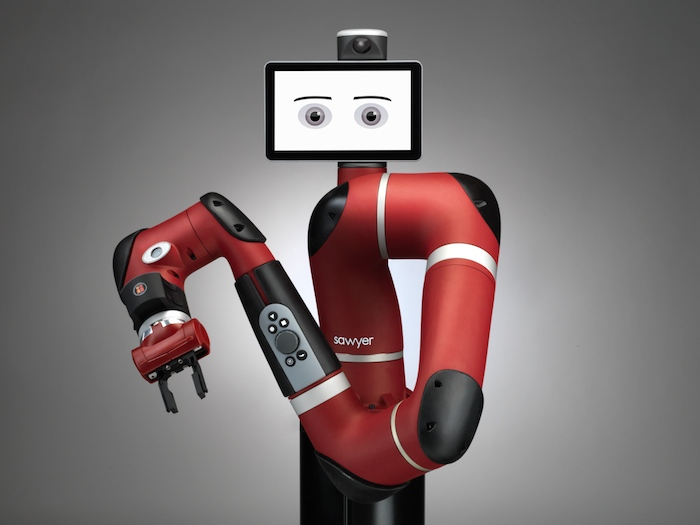
\includegraphics[width=0.5\linewidth]{./img/sawyer.jpeg}
  \caption{Rethink Robotics$^\circledR$ Sawyer\texttrademark}
  \label{fig:sawyer}
\end{figure}%

Dentre os seus diferenciais destaca-se seu peso de apenas $19Kg$, atuadores \textit{Harmonic Drive} com encoder óptico, que garantem maior precisão e repetibilidade, e o \textit{software} Intera baseado em ROS(Robot Operating System). Essas características tornam o Sawyer\texttrademark um sistema promissor para aplicações de robótica em instalações \textit{offshore}.

\subsection{DORIS}
O projeto DORIS, desenvolvido pelo laboratório LEAD-GSCAR, da Universidade Federal do Rio de Janeiro, introduz um sistema robótico onde vagões guiados por trilhos carregam diversas câmeras, sensores e dispositivos para monitorar e inspecionar diferentes áreas e equipamento na parte \textit{topside} de plataformas \citep{nunes2013doris, galassi2014doris, freitas2015embedded}.

As tarefas desse robô consistem principalmente em: monitorar perfis de temperatura utilizando câmeras térmicas infravermelhas, supervisão de pessoal não autorizado, detecção de anomalias sonoras utilizando microfones, detecção de vazamentos de gás com sensores de hidrocarbonetos, inspeção de padrões de vibração de maquinário crítico, interação com interfaces \textit{touchscreen} na plataforma, processamento de dados coletados, armazenamento e transmissão de áudio e vídeo em tempo real.

A interação com o robô é feita através de um \textit{software} chamado de RobotGUI, também desenvolvido pela equipe do LEAD-GSCAR. Através dele o operador é capaz de visualizar dados dos diversos sensores, reproduzir a transmissão de áudio e vídeo, enviar comandos de controle e configurar parâmetros, através de uma interface gráfica customizável. 

\begin{figure}[!ht]
\centering
  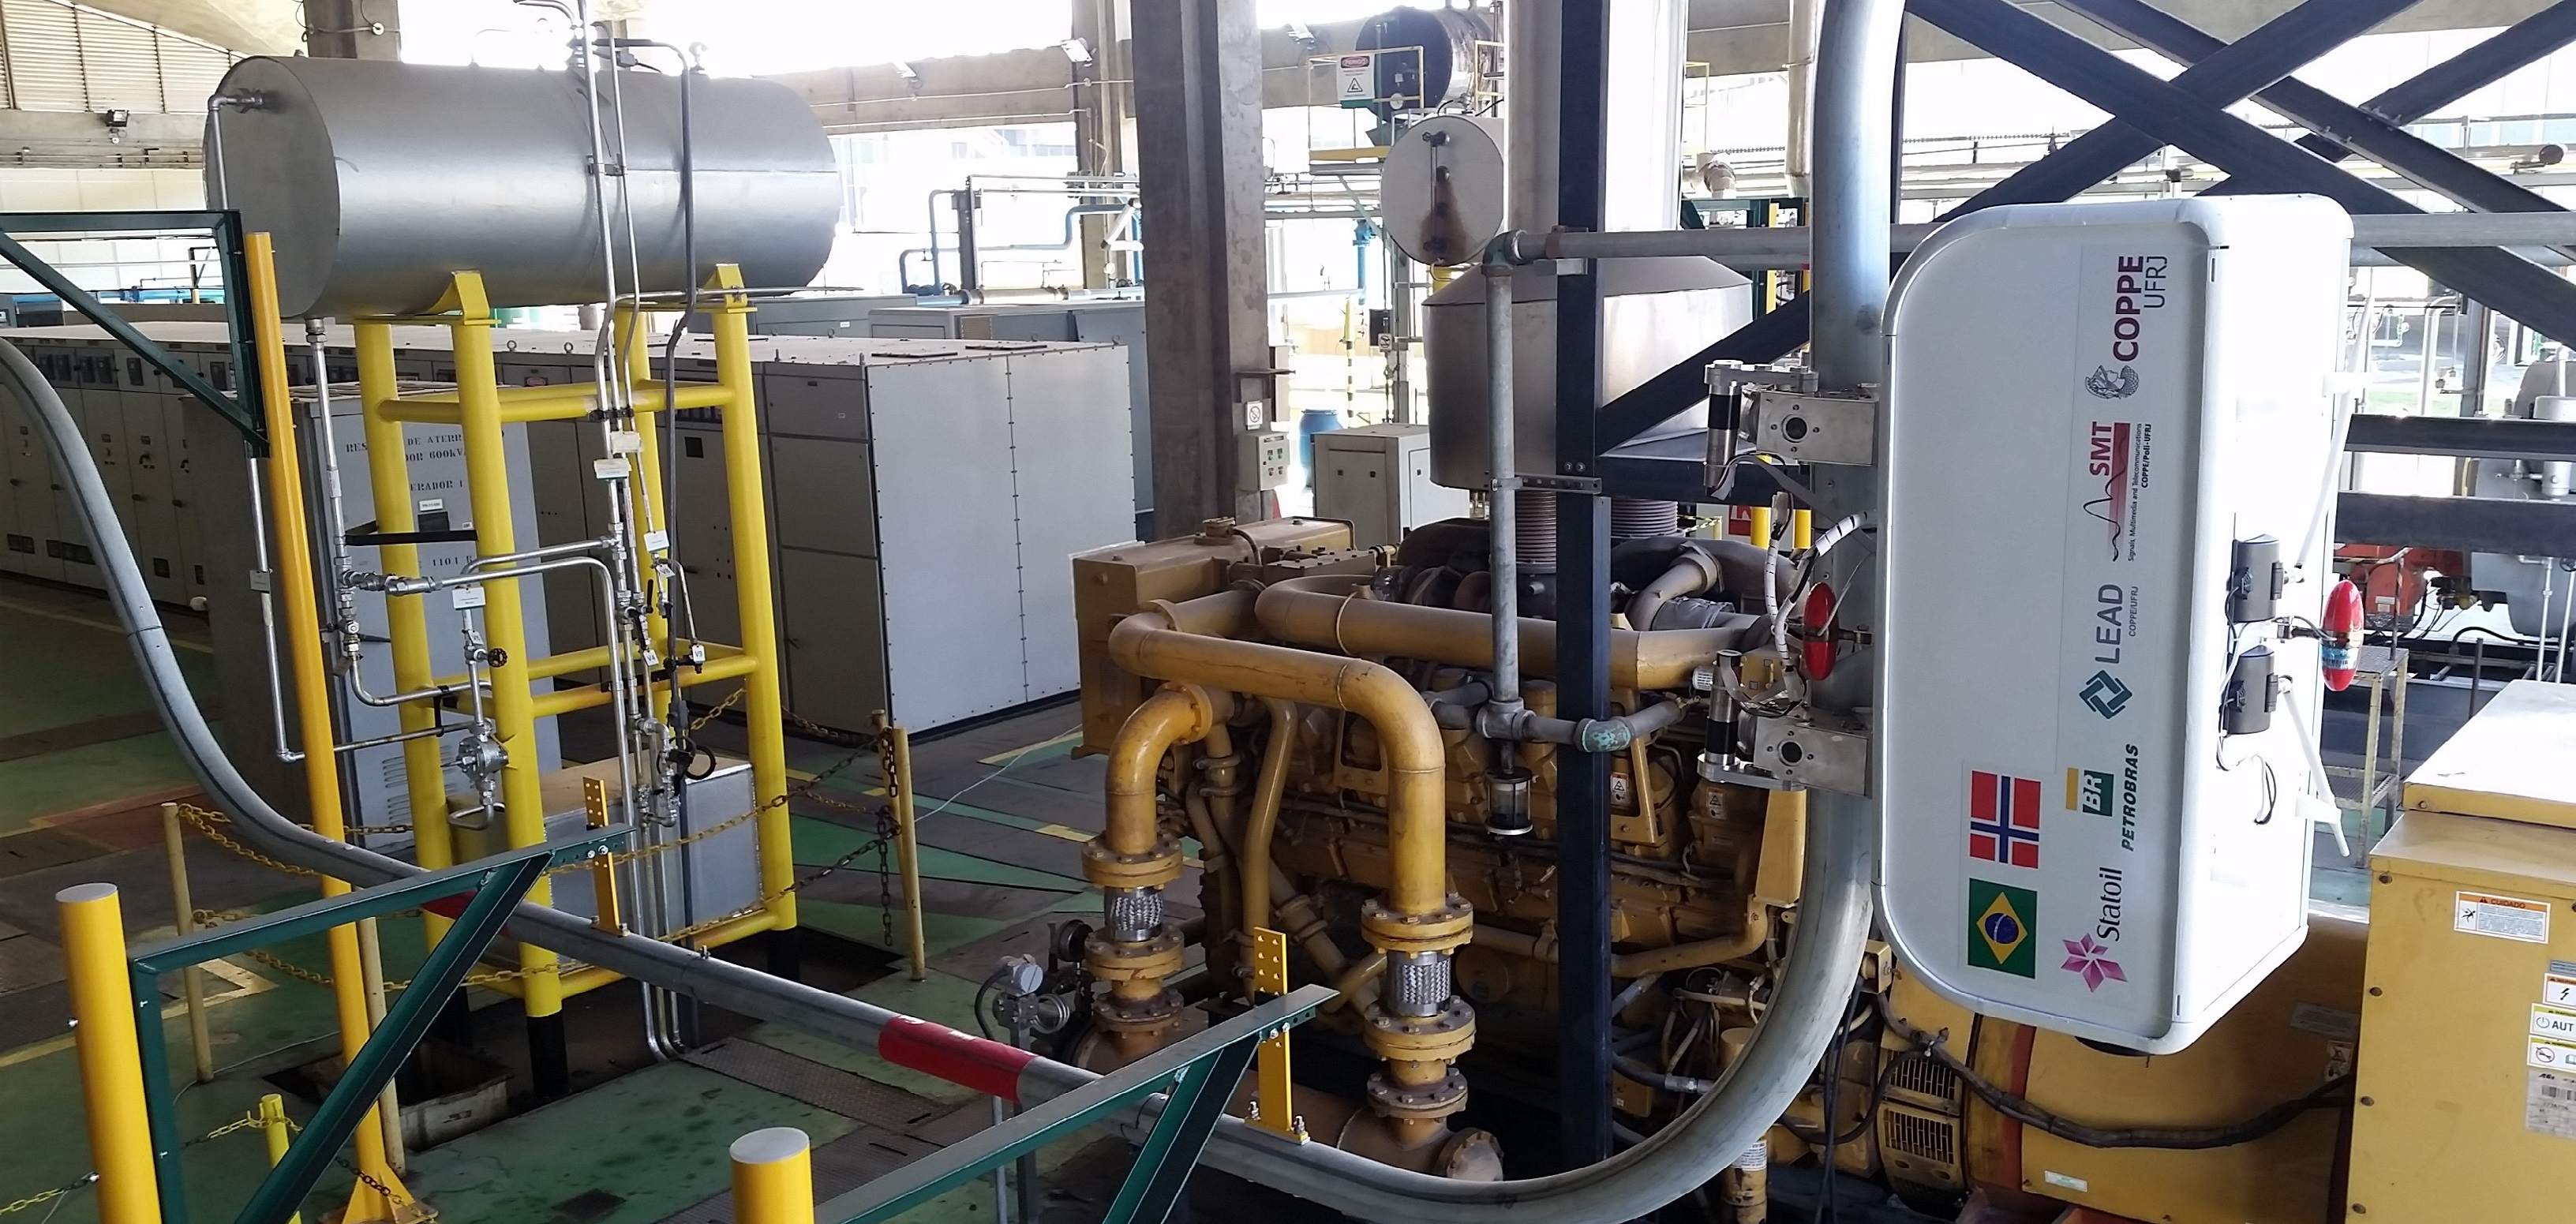
\includegraphics[width=\linewidth]{./img/cenpes_field.jpg}
  \caption{DORIS em operação no CENPES}
  \label{fig:cenpes_doris}
\end{figure}%

\subsection{Manipulador TETIS}
Considerando as tarefas mencionadas foi proposta a adição de um manipulador leve, de modo a extender o espaço de trabalho do robô. Com esse manipulador, pretende-se solucionar os problemas de
\begin{itemize}
\item mover a câmera acoplada ao efetuador, de modo a posicioná-la melhor ao longo da instalação,
\item posicionar um sensor de vibração corretamente sobre a superfície de um equipamento na plataforma e
\item interagir com \textit{touchscreens}.
\end{itemize}

Foi dado a esse manipulador o nome TETIS. O projeto mecânico permite que ele assuma configurações de juntas diferentes, como mostra a Figura \ref{fig:tetis}. 

\newlength{\twosubhtt}
\newsavebox{\twosubboxt}

\begin{figure}[htp]
% preliminary
\sbox\twosubboxt{%
  \resizebox{\dimexpr.9\textwidth-1em}{!}{%
    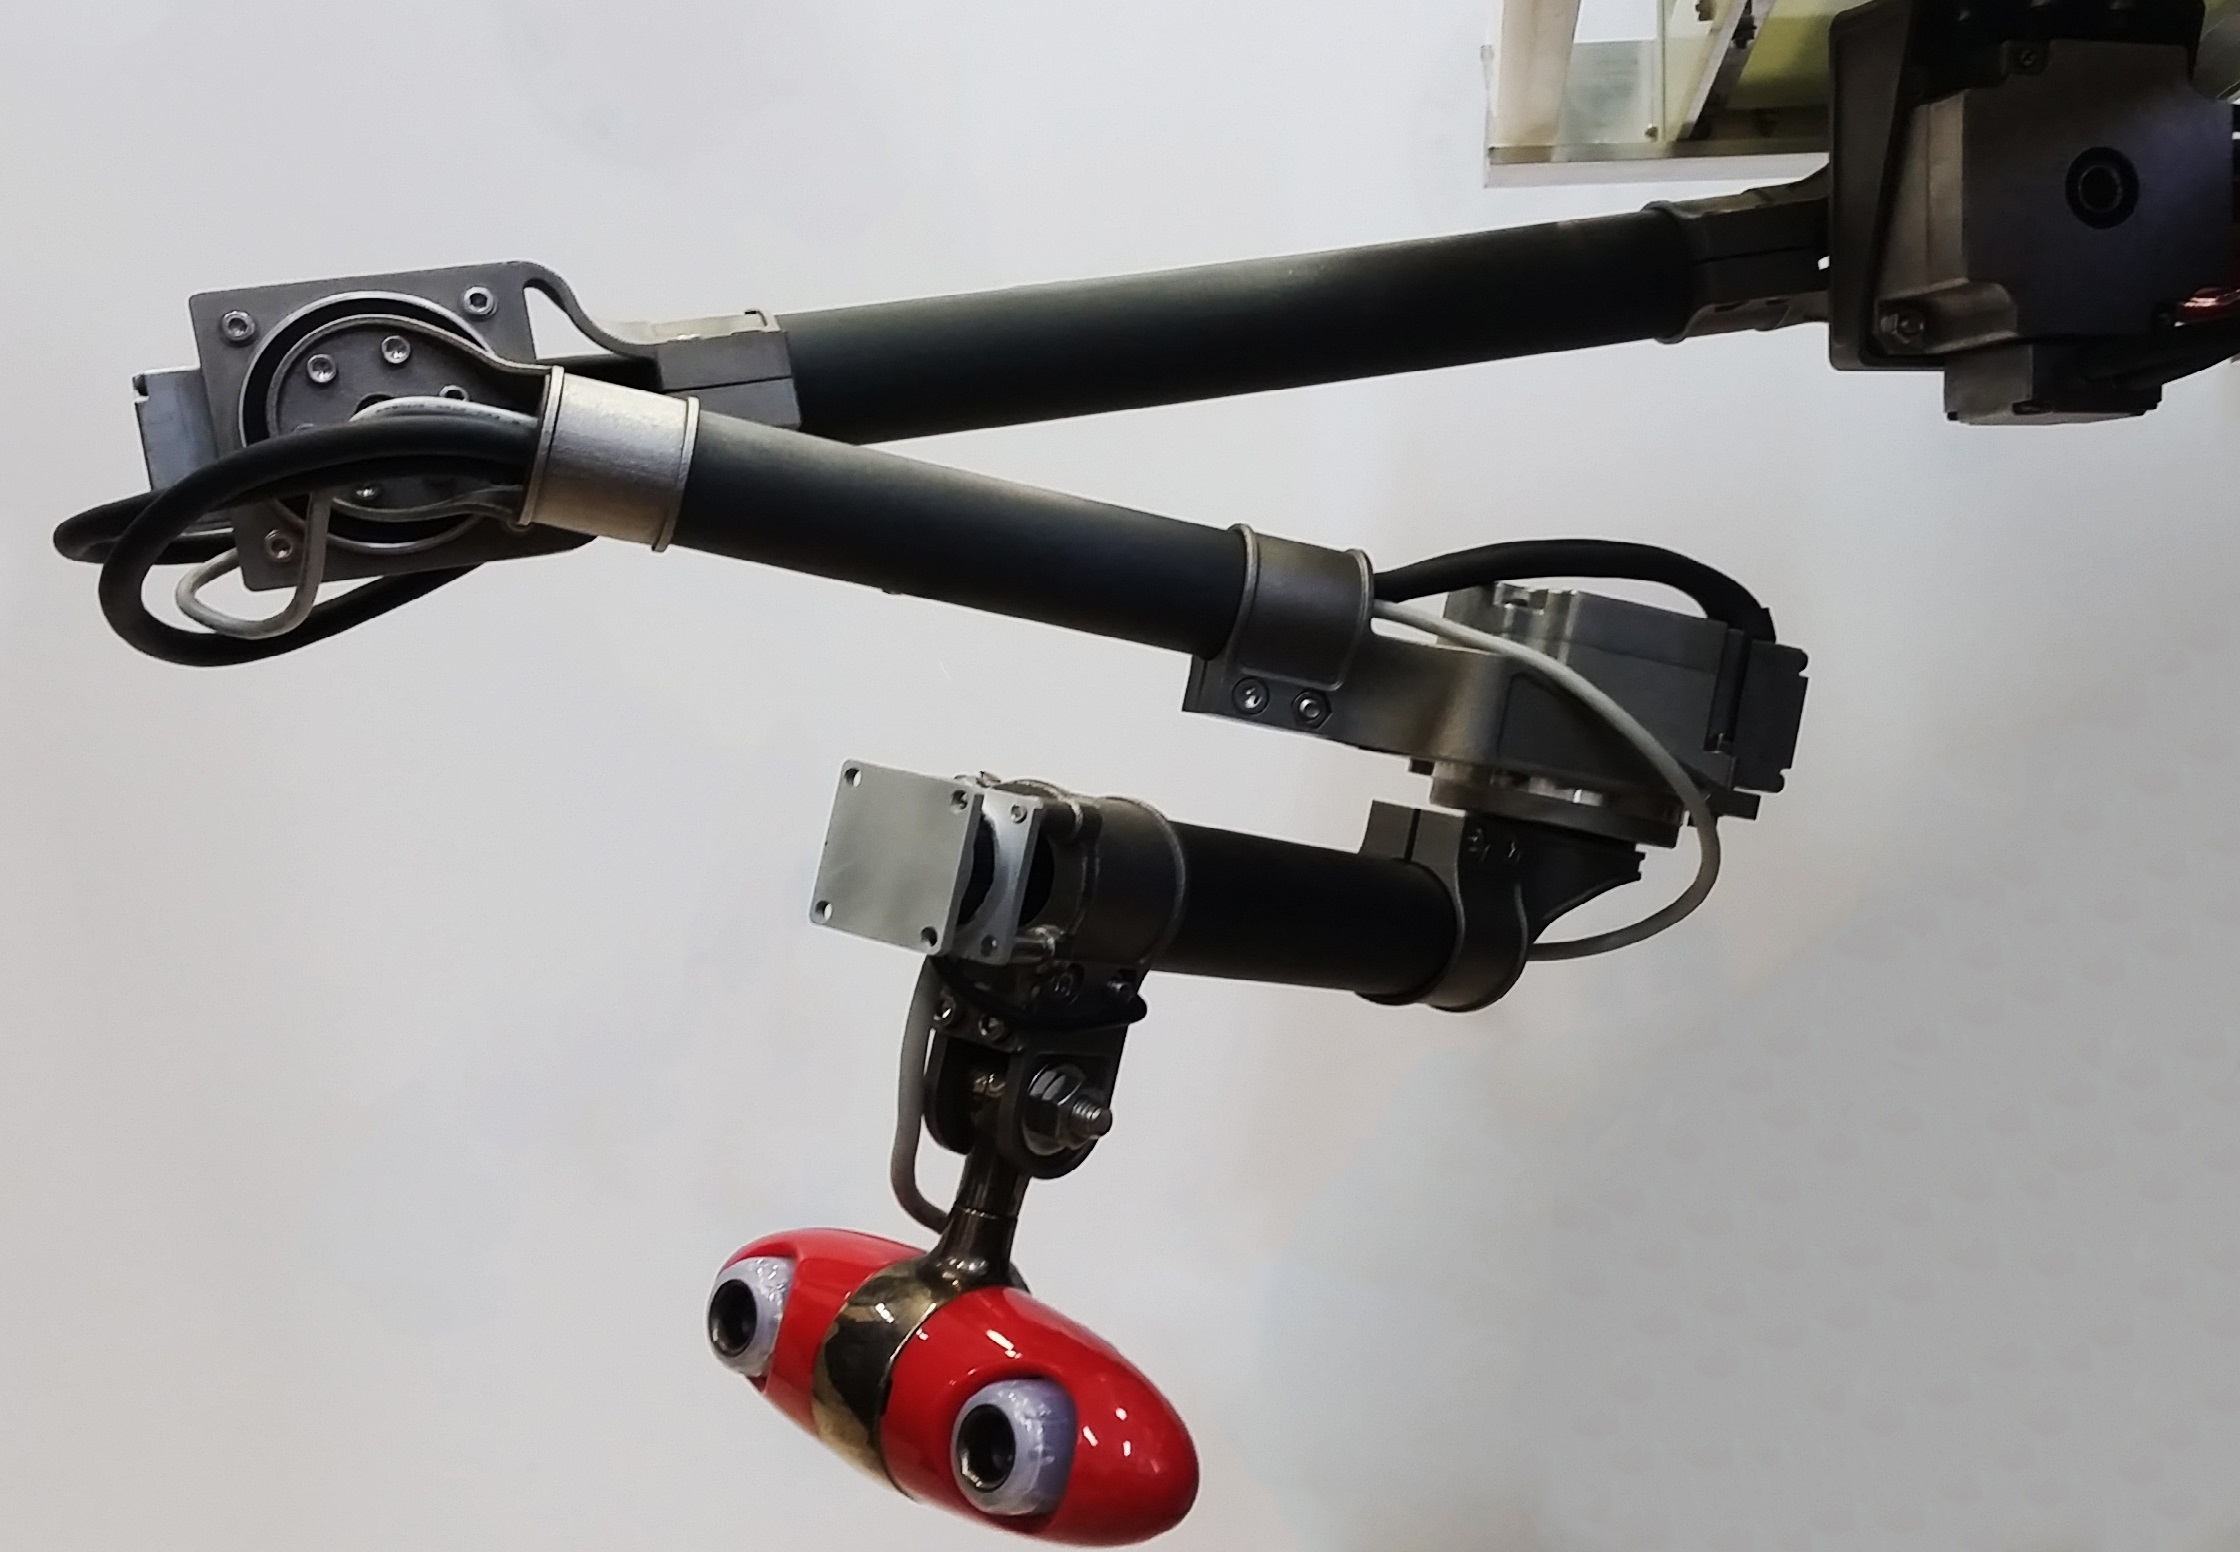
\includegraphics[height=3cm]{./img/manip.jpg}%
    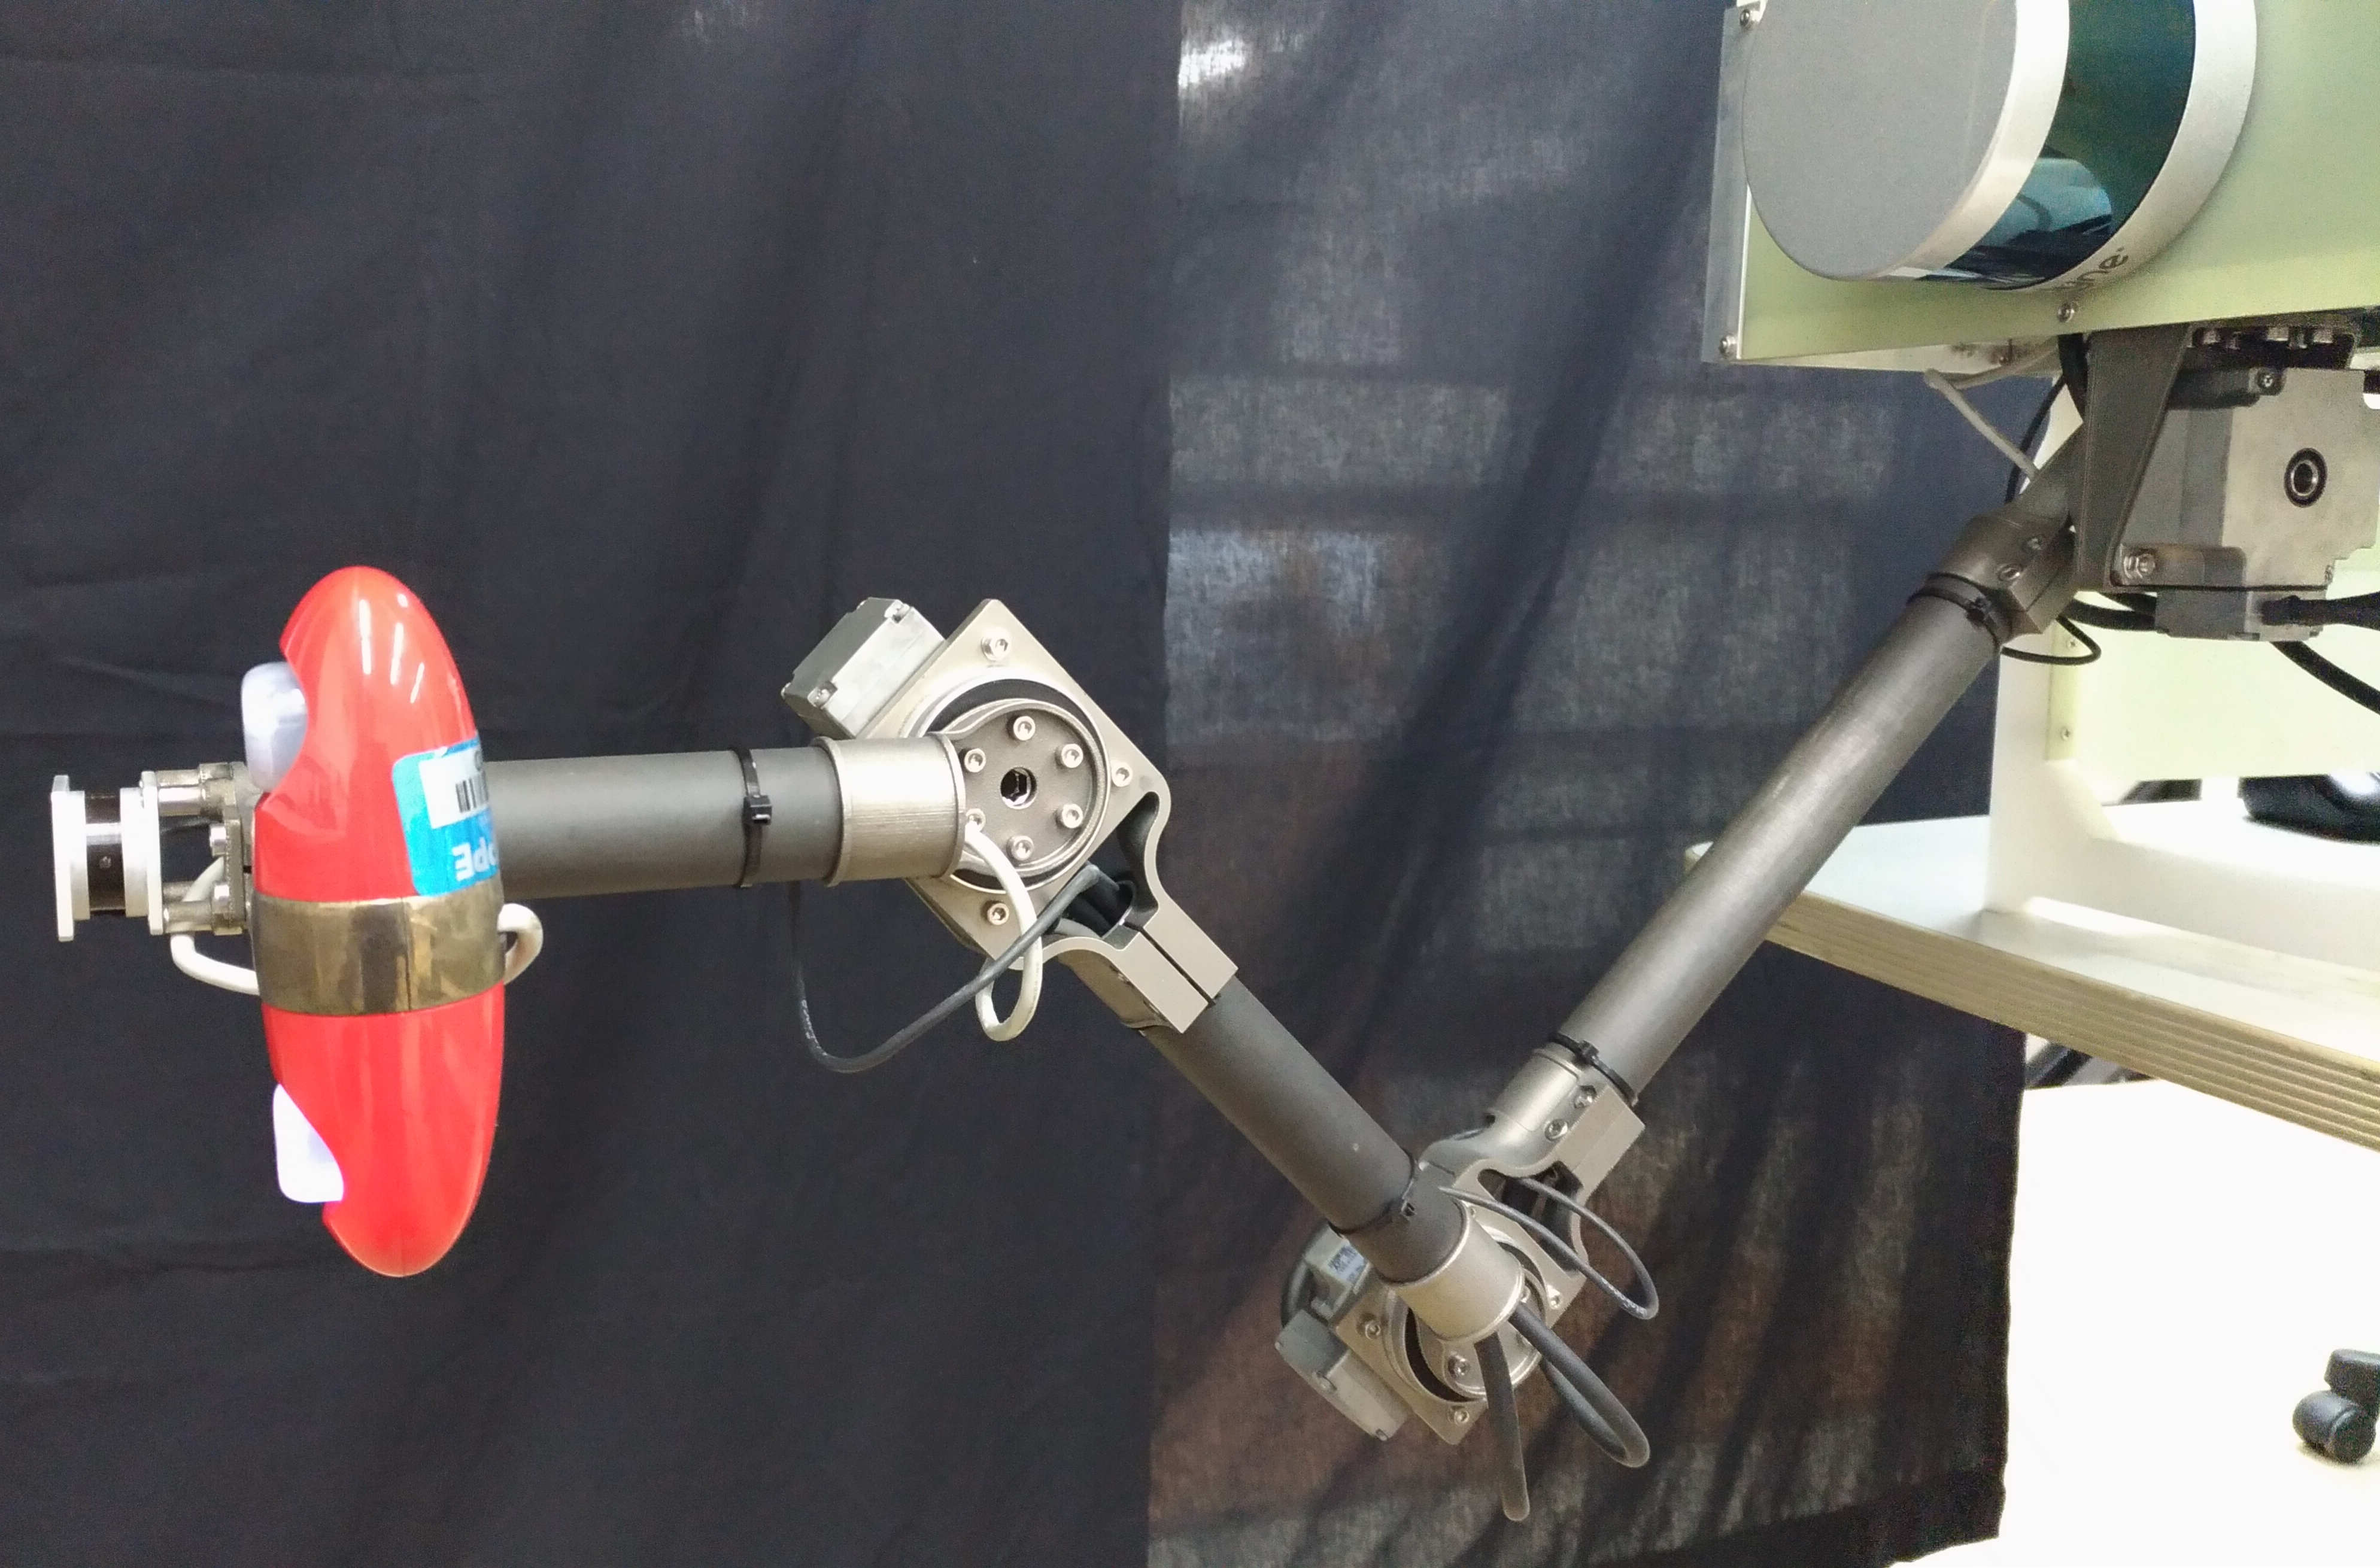
\includegraphics[height=3cm]{./img/manip2.jpg}%
  }%
}
\setlength{\twosubhtt}{\ht\twosubboxt}
% typeset
\centering
\subcaptionbox{Configuração 1\label{fig:tetis1}}{%
  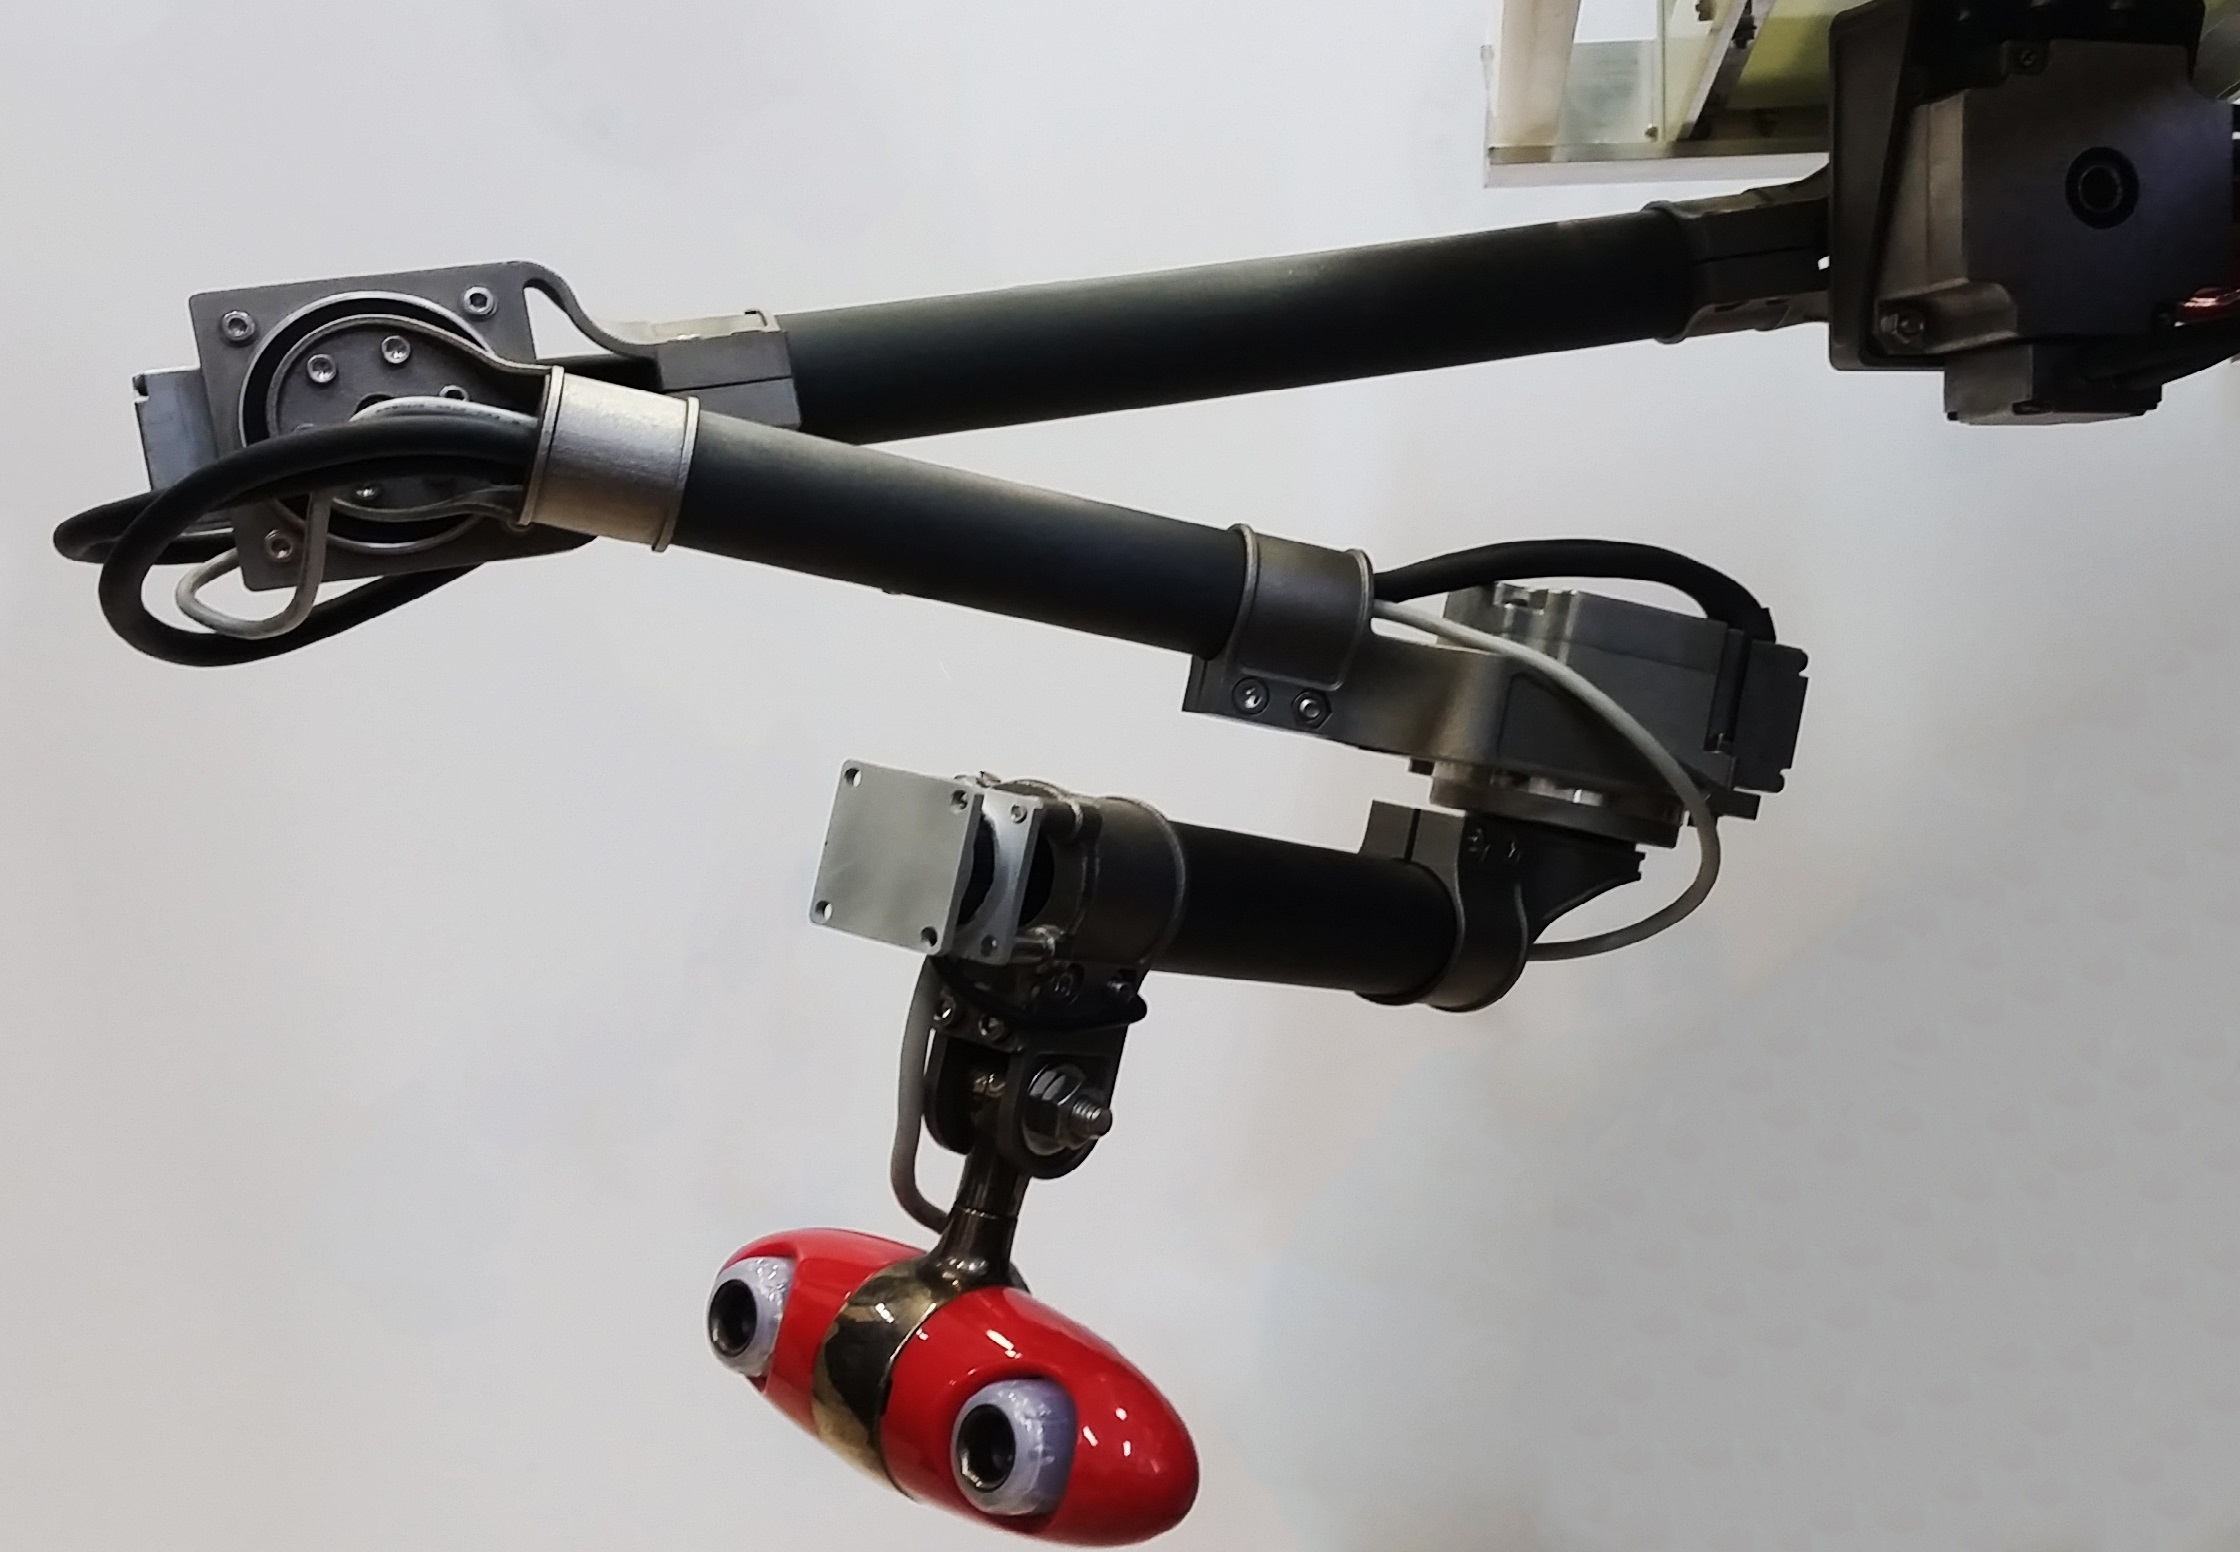
\includegraphics[height=\twosubhtt]{./img/manip.jpg}%
}\quad
\subcaptionbox{Configuração 2\label{fig:tetis2}}{%
  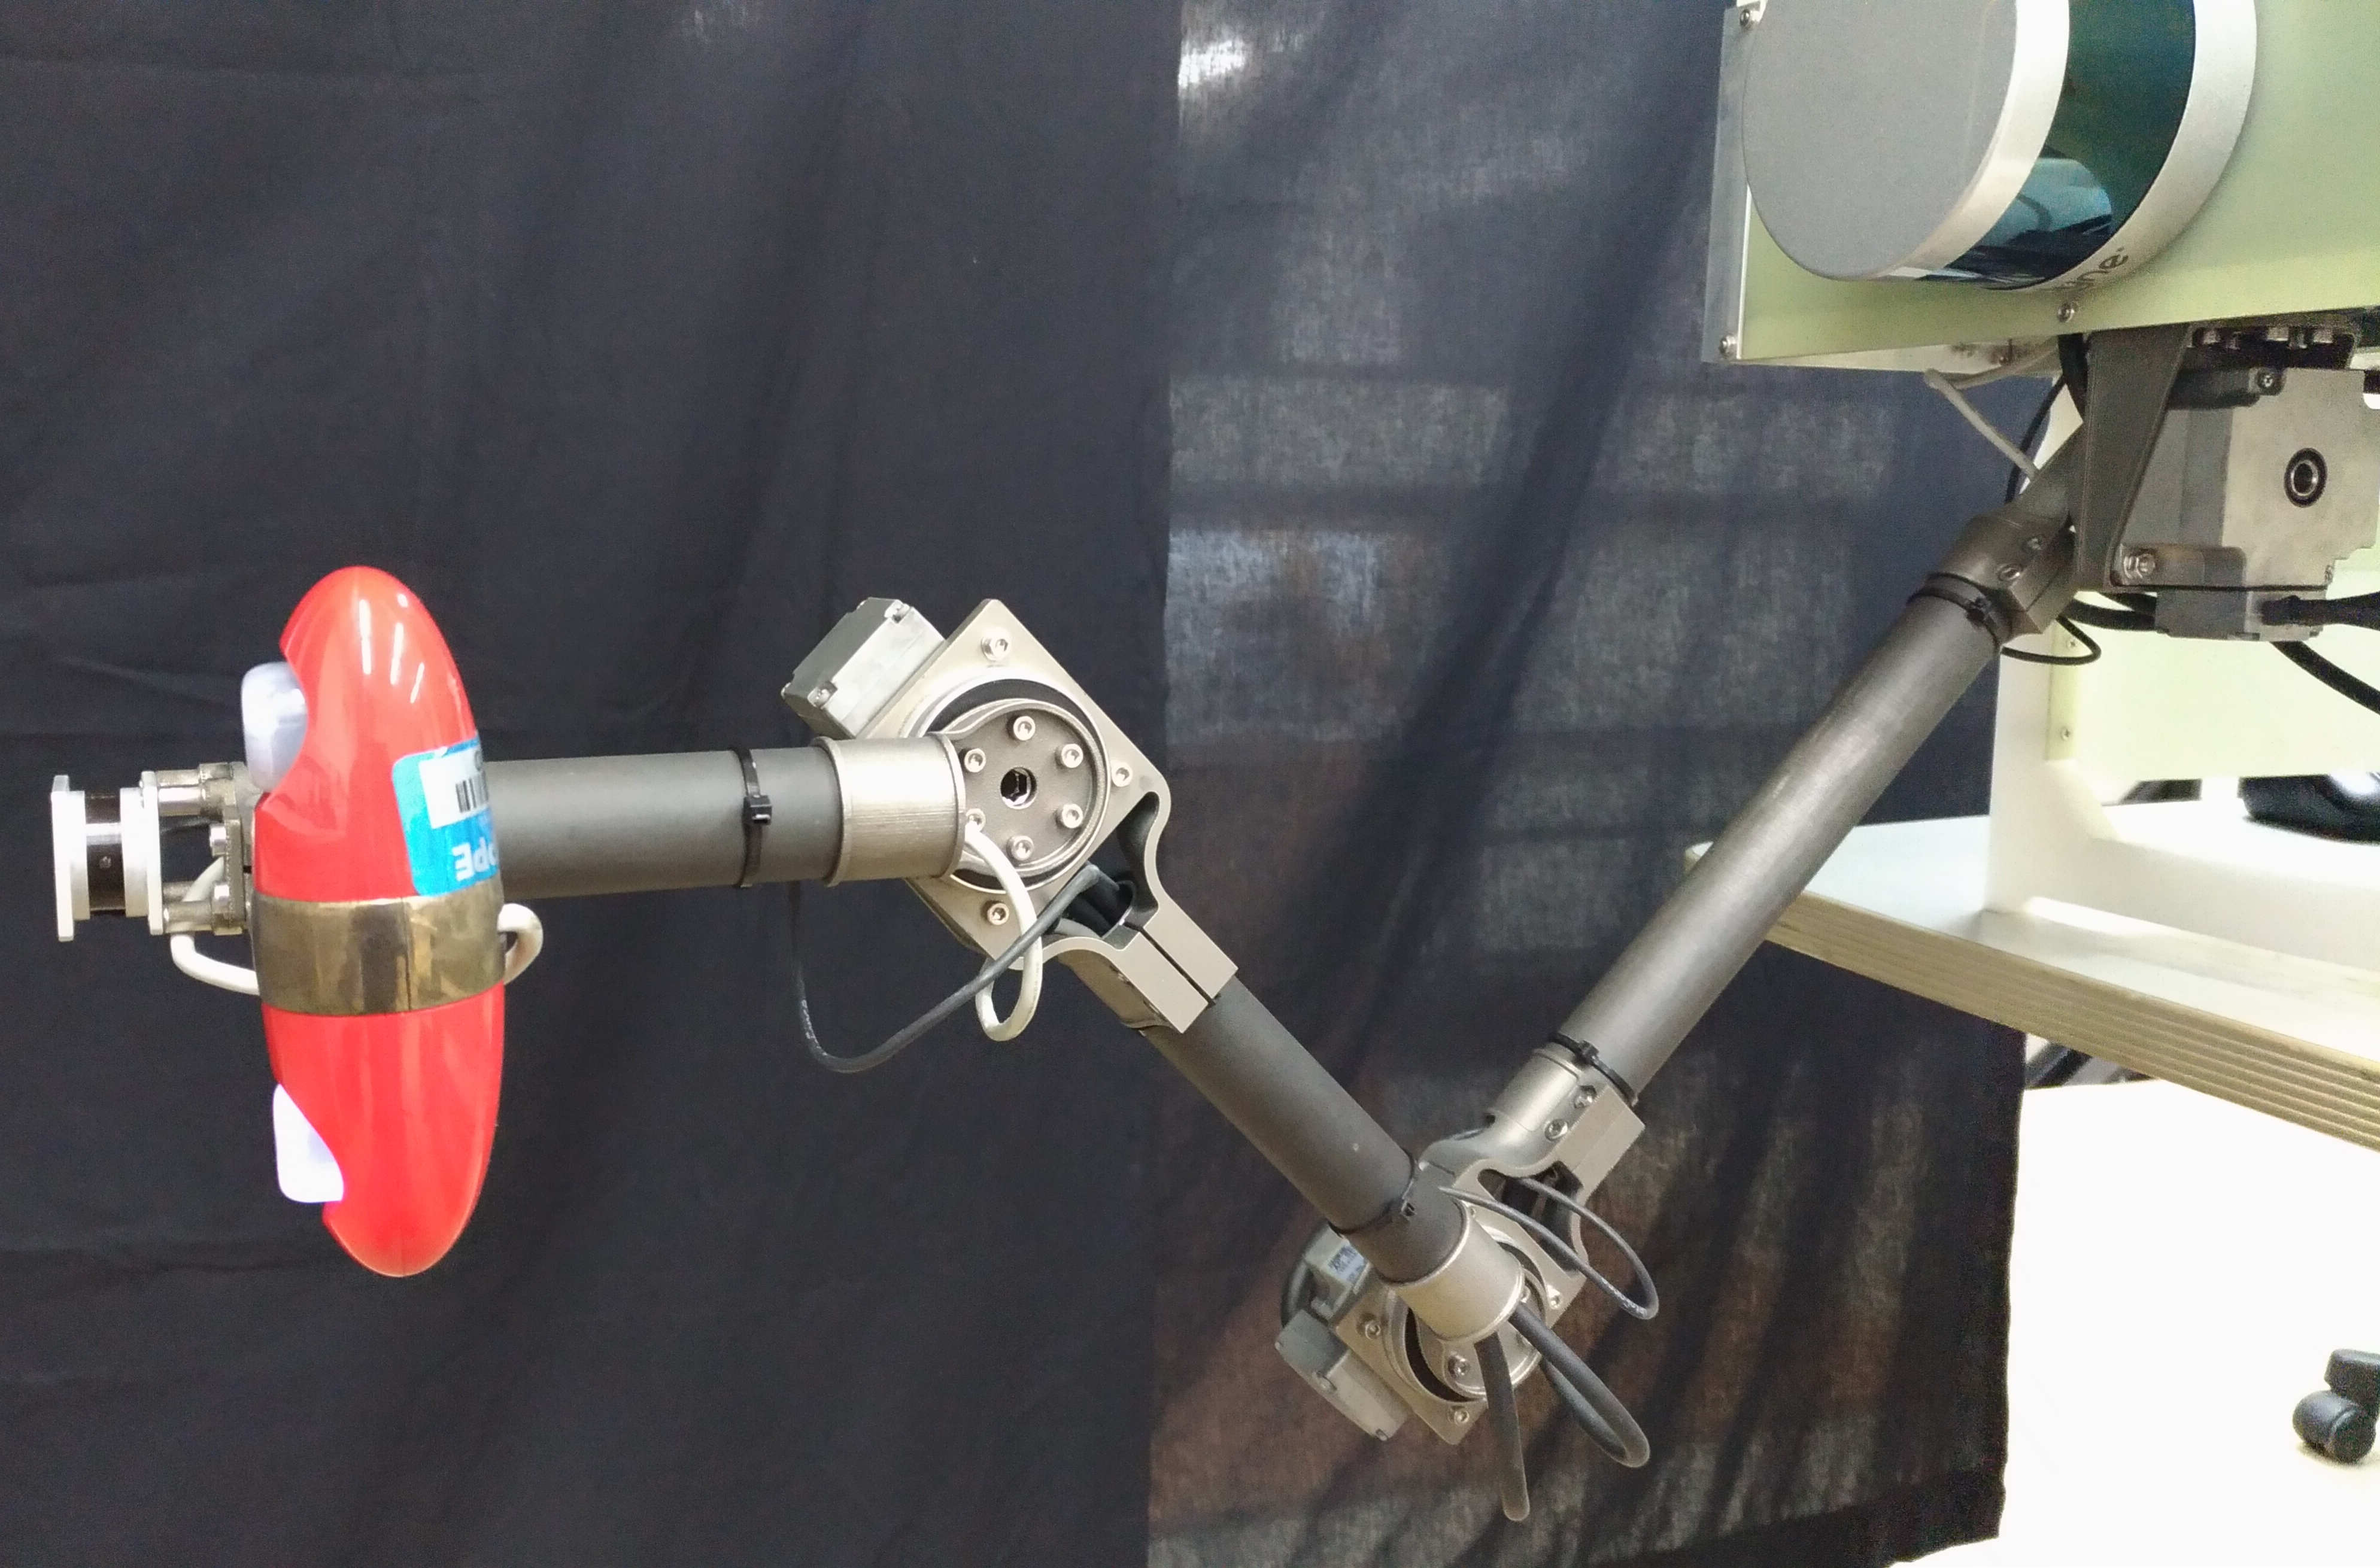
\includegraphics[height=\twosubhtt]{./img/manip2.jpg}%
}
\caption{Manipulador TETIS}
\label{fig:tetis}
\end{figure}

\subsection{Robot Operating System}
Com sua primeira versão em 2007, o \textit{framework} ROS (Robot Operating System) tem ganhado grande aceitação da comunidade para construção de aplicações para robôs. Consiste em um conjunto de bibliotecas e ferramentas que auxiliam no desenvolvimento de \textit{software} para robótica. Essa não é uma tarefa simples, pois o cada vez mais o escopo dos projetos aumenta, englobando algoritmos de controle, visão computacional, percepção e tomada de decisão, entre outros.
 %em projetos de robótica.
Dentre as principais filosofias adotadas, destaca-se a modularidade. 
Muitos projetos tem a tendência de englobar código específico para o robô em questão, de modo que torna-se difícil reaproveitar algorítimos úteis. O ROS encoraja a comunidade de contribuidores a desenvolver pacotes que possam ser reutilizados em outros projetos.  

Processos que utilizam ROS são chamados de nós e comunicam entre si através de uma topologia ponto-a-ponto, podendo ser executados na mesma máquina ou em diferentes computadores em uma LAN. Dessa forma, os diferentes componentes necessários para o \textit{software} de um robô podem ser encapsulados em nós, o que garante uma maior possibilidade de reaproveitamento, facilidade de alteração e versatilidade de execução.


\section{Objetivos}
A partir do projeto mecânico e eletrônico do manipulador finalizado, segue a etapa de modelagem e implementação de estratégias de controle. 
Nesse contexto, insere-se este trabalho. Utilizando a configuração do manipulador mostrada na Figura \ref{fig:tetis2}, alternativa àquela abordada em \citep{xaud2016doris},  busca-se:
\begin{itemize}
\item Elaborar o modelo cinemático e implementar estratégias de controle. %de posição, rastreamento de trajetória.

\item Utilizar a câmera para controle por servovisão onde o alvo é um marcador em algum ponto de interesse, como por exemplo uma máquina a ser inspecionada. 

\item Com o sensor de força montado no efetuador do manipulador, realizar controle de força sobre uma superfície de restrição suave de geometria conhecida.

\item A partir do RobotGUI, que já interage com os outros dispositivos do DORIS, desenvolver um \textit{software} para controle de manipuladores robóticos. O uso do ROS proporciona uma maior versatilidade e facilidade para incorporação de novas funcionalidades, em comparação com abordagens tradicionais.

\item Utilizar \textit{Julia Language}, uma linguagem de programação de alto nível e alta performance orientada para computação científica, para permitir que o algoritmo de controle seja modificado em tempo de execução. Essa linguagem possui mecanismos de compilação em tempo de execução, o que dá mais flexibilidade ao programa, sem perder desempenho.
\end{itemize}


\section{Organização do trabalho}

%TODO
No primeiro capítulo o trabalho foi contextualizado, descrevendo os objetivos do projeto DORIS e do manipulador TETIS. No segundo capítulo são mostrados conceitos de robótica necessários para a modelagem e controle de manipuladores robóticos. No capítulo 3 esses conceitos são aplicados ao manipulador TETIS.
No capítulo \ref{chap:descricao_hard} é descrito o hardware do robô DORIS.  No capítulo 5 são abordados detalhes das ferramentas e da arquitetura utilizada para a implementação do \textit{software}. No capítulo 6, são mostrados e discutidos os resultados de simulação e de testes experimentas para os diferentes modos de controle implementados.  Por último, no capítulo 7 são apresentadas as conclusões sobre o trabalho e pontos para serem abordados em trabalhos futuros.

